% !TEX root = ../thesis.tex

\chapter{Analytická časť}

%%---------------------------------------------------------------
\section{Čo je to Internet vecí}
Skôr ako začnete navrhovať a plánovať projekt internetu vecí, musíte najprv pochopiť definíciu internetu vecí a jeho základné princípy.

Takže, čo je to internet vecí? Ak sa spoľahneme na málo spoľahlivý zdroj, konkrétne na Wikipédiu, nájdeme nasledujúcu definíciu:

\textit{Internet vecí (\gls{iot}) označuje fyzické objekty (alebo skupiny takýchto objektov) so senzormi, spracovateľskými schopnosťami, softvérom a ďalšími technológiami, ktoré sa spájajú a vymieňajú si údaje s inými zariadeniami a systémami prostredníctvom internetu alebo iných komunikačných sietí.}\cite{wiki}

Môžem povedať, že táto definícia celkom dobre vystihuje základnú myšlienku tohto pojmu, ale myslím si, že jej chýba konkrétnosť. Čo sa týka akademickej definície internetu vecí, v tejto oblasti neexistuje vedecký konsenzus. Vo všeobecnosti si rôzni akademici definíciu mierne upravujú po svojom, ale ak to zhrnieme, najlepšia definícia by bola takáto:

\textit{An open and comprehensive network of intelligent objects that have the capacity to auto-organize, share information, data and resources, reacting and acting in face of situations and changes in the environment.}\cite{book}

Ďalším dôležitým aspektom porozumenia \gls{iot} je to, že je to sieť inteligentných zariadení, ktoré si vymieňajú dáta a táto sieť má svoju hierarchiu a logiku. To znamená, že jedno chytre zariadenie, aj keď má nejaký softvér a vykonáva konkrétnu úlohu (napríklad smartphone), nie je \gls{iot}, kým ho nepripojíte k sieti a nedáte mu konkrétnu úlohu v tejto sieti. Ako som už písal, sieť má svoju hierarchiu, ale pre štandardizáciu a koordináciu rôznych vývojov musí byť premyslená na základe nejakej architekturnej konceptuálnej modely. Napríklad v sieti Internet sú také konceptuálne modely, ako \textit{OSI} a \textit{TCP/IP}. V rámci \gls{iot} je tiež podobná architekturna model. Pokiaľ ide o vzhľad tejto modely, vedecká spoločnosť opäť nemá konsenzus. Na internete nájdete veľa rôznych architektúr s rôznymi počtami vrstiev a názvami, ale všetky majú približne rovnaký význam. V ďalšej práci budem používať architektonický model, ktorý sa skladá zo štyroch vrstiev.

\begin{figure}[!ht]
    \centering
    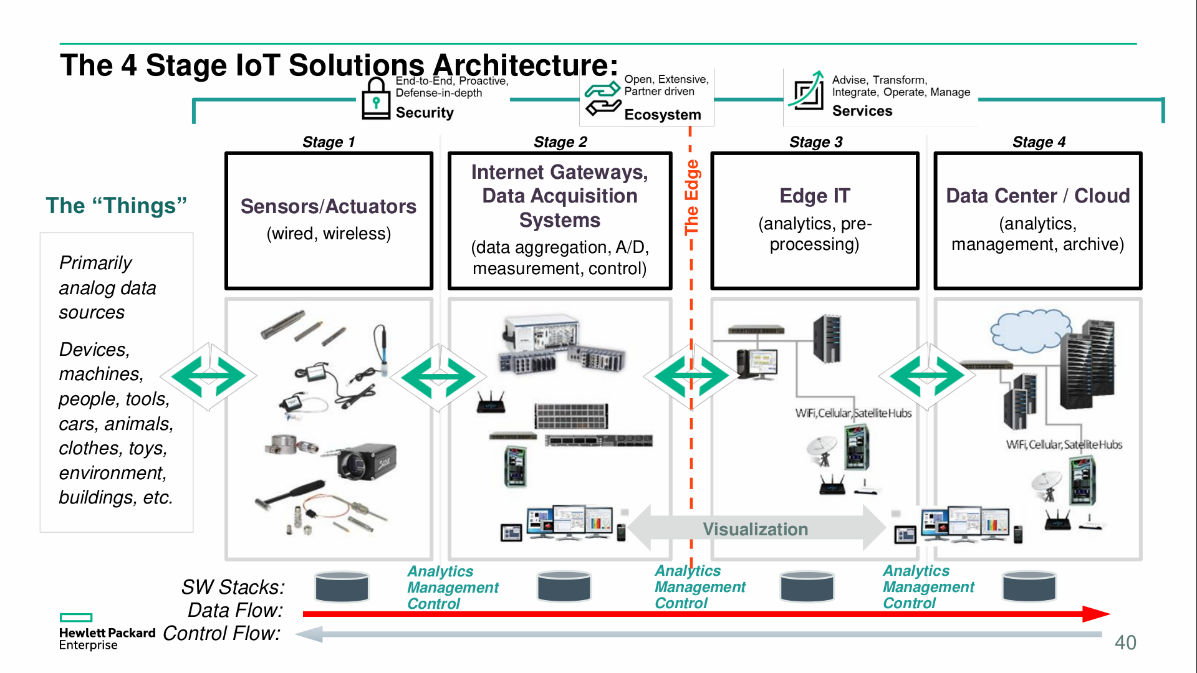
\includegraphics[width=.9\textwidth]{figures/iot}
    \caption{Vrstvy architektúry \gls{iot} riešení \label{iot} \cite{iotTukeLekcia1}}
\end{figure}

Zoznam jednotlivých vrstiev tohto modelu (obr. \ref{iot}) je nasledový:

\begin{itemize}
    \item \textit{Prvá vrstva}: Táto vrstva obsahuje snímače údajov a rôzne elektrické pohony na interakciu s prostredím. Môžu komunikovať s vyššou vrstvou aj medzi sebou. Objekty na tejto vrstve nemusia byť \textit{inteligentné} (napríklad DHT 11, motorček, mikrokontrolér).
    \item \textit{Druhá vrstva}: Na tejto vrstve sa nachádzajú brány prepojenia systému. Teda zariadenia, ktoré prijímajú údaje z predchádzajúcej vrstvy, poskytujú príkazy pohonov, vykonávajú primárne spracovanie a filtrovanie údajov a majú softvér. Táto úroveň sa zvyčajne fyzicky nachádza veľmi blízko k prvej a je jednou z najdôležitejších úrovní v celej sústave. Na tejto vrstve môže byť aj vizualizácia zozbieraných údajov.
    \item \textit{Tretia vrstva}: Táto vrstva slúži na zber a spracovanie údajov z predchádzajúcej vrstvy a ich pripravenie pre archiváciu alebo pre konečného spotrebiteľa. Zvyčajne táto úroveň slúži na zmiernenie zaťaženia hlavných serverov a na rýchlejšiu odpoveď používateľovi, ale môžu byť výnimky. Tretia vrstva nie je povinná pre použitie v \gls{iot} architektúre.
    \item \textit{Štvrtá vrstva}: Je konečnou vrstvou, na ktorej sa informácie analyzujú, archivujú alebo sa dostanú ku konečnému používateľovi používanie aplikácií.
\end{itemize}

Vychádzajúc z celého vyššie uvedeného, možno povedať, že koncept \gls{iot} a jeho architektúra riešia otázky zberu, spracovania a transportovania dát. Preto pri navrhovaní \gls{iot} riešení treba sústrediť pozornosť práve na správne manipulovanie s dátami.

V svojej prace sa budem snažiť dôsledne predstaviť študentom podstatu teoretického konceptu \gls{iot} a detailne ukázať všetky úrovne architektúry \gls{iot} riešení na príkladoch z praxe.

%%---------------------------------------------------------------

\section{Moje skúsenosti s vyučovaním \gls{iot} a prácou s elektronikou}
V tejto práci sa budem často rozhodovať na základe svojich skúseností, preto si myslím, že pred začatím samotnej analýzy a plánovania je potrebné sa podrobnejšie pozrieť na moje skúsenosti so vzdelávaním v oblasti \gls{iot}. Moje zoznámenie s \gls{iot} sa stalo až nedávno, v treťom ročníku môjho štúdia na univerzite v rámci predmetu \gls{iot}\cite{iotTuke}. Materiál tohto predmetu umožňuje rozšíriť znalosti v oblasti \gls{iot}, zoznámiť sa s jej rôznymi aspektmi, aby sme na konci semestra mohli navrhnúť a vytvoriť produkt na základe tejto koncepcie. Cieľom tohto kurzu je poskytnúť základné znalosti na úrovni junior developera v tejto oblasti. Celkovo som s týmto kurzom spokojný, ale chcem zdôrazniť jeho hlavnú nevýhodu, a to nevyváženosť praktických cvičení. Podľa môjho názoru boli praktické cvičenia viac zamerané na interakciu so systémom \textit{Docker} a menej na prácu s hardvérom. Okrem toho bolo učenie sa práce s hardvérom umiestnené až na konci a to tiež nie je podľa mňa najlepšia myšlienka.

Považujem, že základom \gls{iot} je interakcia s mikrokontrolérmi a mikroprocesormi, preto sa budem snažiť venovať väčšinu praktických úloh práve tejto interakcii. Je možné poznamenať, že \gls{iot} je koncept, ktorý sa stavia na komunikácii, nie na hardvéri.

Chcel by som spomenúť zaujímavú skúsenosť z účasti na workshopu zameranom na zoznámenie sa s \textit{ESP32}. Táto skúsenosť bola veľmi zaujímavá, pretože štruktúra prezentácie na tomto podujatí je tou, ktorú chcem zrealizovať aj vo svojom projekte. Teda, samotný webinár bol postavený takým spôsobom, že po krátkej teoretickej časti nasledovala praktická časť, čo umožňovalo udržiavať pozornosť poslucháčov neustále v strehu. V takomto vzdelávacom prístupe môžem identifikovať iba jednu nevýhodu - problém zaostávajúceho účastníka. Ak študent nestíha doháňať ostatných aspoň na jednej úrovni, bude pre neho veľmi ťažké udržiavať krok s ostatným materiálom.

%%---------------------------------------------------------------
\section{Analýza podobných riešení a cieľovej skupiny projektu.}
\subsection{Analýza riešení na Slovensku}
Pri hľadaní podobných projektov na Slovensku som našiel len veľmi málo referencií. Preto som dospel k záveru, že internet vecí sa na Slovensku veľmi nerozvíja. Jediný skutočne podobný kurz sa organizoval na \textit{Strednej odbornej škole elektrotechnicky v Žiline}\cite{slovakKurz}. Materiály celého kurzu nie sú bohužiaľ \textit{open sorse}, preto som analyzoval dostupné informácie z ich webovej stránky a reportáže. Po ich preskúmaní som si všimol, že to je presne to, čo sme potrebovali. Ak som pochopil z dostupných útržkov informácií, tento týždňový kurz bol rozdelený do dvoch skupín: \textit{Robotika} a \textit{}. \gls{iot}

Počas kurzu študenti pracovali s hardvérom, inštalovali potrebný softvér pre prácu a, samozrejme, programovali, a to je presne to, čo chcem implementovať do svojej práce. 

Moje tvrdenie vychádza z faktu, že všetky komponenty sa dajú kúpiť s prispájkovanými pinmi a takéto komponenty sa cenovo minimálne líšia od bežných riešení.

Veľkou nevýhodou tohto kurzu je, že všetky jeho materiály nie sú zdokumentované a zverejnené na internete.  To neumožní opätovné vytvorenie tohto kurzu alebo jeho samostatné zvládnutie. Preto si myslím, že by bolo správne sprístupniť môj projekt čo najväčšiemu počtu ľudí, čiže umiestniť všetky študijné materiály na internet.

%%---------------------------------------------------------------

\subsection{Analýza medzinárodných riešení}
Naozaj prekvapujúco som na internete našiel mnoho rôznych kurzov \gls{iot} v angličtine. Existujú rôzne typy kurzov, platené a bezplatné, ale väčšina z nich je zameraná na dospelú populáciu. Môžem uviesť niekoľko zaujímavých riešení pre školy.

Prvým je výučbový kurz od spoločnosti \textit{Cisco}\footnote{\textit{https://www.cisco.com/}} s názvom \textit{Introduction to} \gls{iot} \cite{ciscoKurz}. Je zaujímavý tým, že prebieha úplne online a môže ho absolvovať hocikto bez učiteľa. Avšak, tento kurz má dosť problémov, napríklad, že sa v ňom nachádza prevažne len teoretická časť. Z praktických cvičení sú tam len testy na overenie znalostí a ich odpovede možno ľahko nájsť na internete. Preto sa mi zdá, že kurz nie je kompletný. 

Spoločnosť \textit{Cisco} sa snažila tento problém riešiť spoluprácou s univerzitami. Príkladom takej spolupráce je kurz s názvom \gls{iot} \textit{Step by Step 2021}\cite{educInit}. V tomto študijnom programe sa kurz od \textit{Cisco} používa iba ako teoretický základ, po jeho dokončení deti prechádzajú na praktickú časť. To je príklad dosť dobreho riešenia tohto problému.

Ďalšou prácou, na ktorú by som chcel upozorniť, je kurz \textit{Internet of Things Education Package}\cite{educPac} od spoločnosti \textit{Software AG}. V tomto kurze je jedno originálne riešenie, o ktorom by som chcel napísať, a to o možnosti použitia svojho smartfónu ako stanice zberu dát pre svoj \gls{iot} projekt. Toto je jednoduché a geniálne riešenie zároveň. Študentom nie je potrebné poskytovať ďalšie zariadenie na zber dát a nemusia navrhovať a testovať svoje riešenie, pretože v súčasnosti každý má smartfón, ktorý má všetky potrebné základné senzory. Preto takéto riešenie veľmi šetrí čas, vzdelávanie a peniaze. Pri vývoji svojho kurzu zvážim možnosť implementácie takéhoto riešenia.

Zhrnutím môžem povedať, že väčšina bezplatných, medzinárodných produktov, ktoré som našiel, sú dosť zaujímavé na štúdium. Žiaľ, nemohol som vidieť, ako tieto kurzy prebiehali, a nenašiel som ani recenzie používateľov, ale myslím, že som bol schopný pochopiť architektúru školenia a informácie, ktoré tieto kurzy poskytujú. Hoci sa tieto výučbové kurzy líšia od toho, čo chcem urobiť, zohľadním informácie, ktoré som získal v rámci prípravy tejto analizy.

%%---------------------------------------------------------------

\subsection{Analýza znalostí študentov stredných škôl na Slovensku}
Pred začatím vývoja kurzu je potrebné uvedomiť si úroveň znalostí, ktoré majú študenti. V našom prípade sú to študenti stredných škôl na Slovensku. Keďže som nedosiahol stredné vzdelanie na slovenských školách, priamo nebudem schopný posúdiť znalosti, ktoré tieto školy poskytujú. Preto som sa opýtal niekoľko svojich známych a priateľov, ktorí sa učili na slovenských školách.

Zaujímali ma tieto otázky:
\begin{itemize}
    \item Rozsah tém, ktoré študenti stredných škôl preberajú v predmete informatika.
    \item Kvalita znalostí, ktoré získavajú študenti.
    \item Možné špecifikácie vzdelávania.
\end{itemize}
Na základe tohto prieskumu môžem povedať, že cieľová skupina môjho kurzu by už mala vedieť:
\begin{itemize}
    \item Základy programovania.
    \item Základy práce s doskou Arduino Uno.
\end{itemize}
S ohľadom na vyššie uvedené parametre možno dospieť k záveru, že táto znalostná báza umožní neplýtvanie časom na vysvetľovanie elementárnych vecí z oblasti programovania/elektroniky a umožní sa sústrediť na zložitejšie veci. Chcem poznamenať, že nemôžem presne vedieť úroveň znalostí každého potenciálneho študenta, preto budem vychádzať práve z vyššie uvedených zaverov.

%%---------------------------------------------------------------
\section{Podrobné plánovanie projektu a jeho jednotlivých častí}
\subsection{Základné princípy}
Pri vývoji tohto projektu sa chcem držať týchto princípov:
\begin{enumerate}
    \item \textit{Dostupnosť} - hlavný princíp. Pretože práve ona umožní dostať informácie k väčšiemu množstvu ľudí, keďže popularita je hlavnou hodnotou toho, čo robíme v ére internetu. Dostupnosť zahŕňa nasledujúce aspekty:
    \begin{itemize}
        \item \textit{Open source} - Všetka vykonaná práca a všetky údaje musia byť voľne dostupné. To umožní akémukoľvek záujemcovi reprodukovať alebo doplniť moju prácu. Projekt musí mať dobrú dokumentáciu.
        \item \textit{Cenovo dostupné} - Všetky zariadenia musia byť maximálne dostupné a lacné. V ideálnom prípade, ak by všetky potrebné zariadenia pre kurz boli súčasťou štandardného zariadenia \textit{Arduino Kit}, pretože už je k dispozícii takmer vo všetkých stredných školách na Slovensku. Ale je dôležité pochopiť, že kvalita kurzu je prioritnejšia ako nizka cena, takže ak je to potrebné, budem vyberať drahšie zariadenia.
    \end{itemize}
    \item \textit{Kvalita informácií} - Kurz musí obsahovať len to, čo je skutočne potrebné a musí byť maximálne užitočný pre svoju cieľovú skupinu.
    \item \textit{Atraktivita} - Študent nesmie byť nudný počas výučby. Tento princíp je pomerne subjektívny, takže neviem, či ho dokážem uplne splniť.
\end{enumerate}
Verim vieru, že dodržaním týchto zásad môžeme vytvoriť dobrý produkt, ktorý sa môže ďalej zdokonaľovať. Preto sa môj ďalší postup môže odkazovať práve na tieto body.

%%---------------------------------------------------------------

\subsection{Moja vízia projektu a jeho plánovania}
Z kontextu úlohy a počas prvých konzultácií s veducim tejto bakalárskej práce, som pochopil, že konečným cieľom tohto projektu je vytvorenie \gls{iot} produktu študentami a počas tejto vývojovej práce sa študenti naučia základy \gls{iot}.

Mojimi hlavnými úlohami ako vývojára tohto projektu sú:
\begin{itemize}
    \item Vymyslieť a vyrobiť konkrétny \gls{iot} produkt.
    \item Rozdeliť vývoj tohto produktu na niekoľko častí, ktoré budú základom pre lekcie.
\end{itemize}
V ďalšej časti podrobnejšie opíšem oba kroky tejto práce.

Počas dlhých rozhovorov o tom, ako by mal projekt vyzerať, som dospel k záveru, že produkt, ktorý budú deti vyvíjať, by mal byť zaujímavý a názorný v používaní. To znamená, že študenti by mali byť schopní ľahko overiť fungovanie svojho výrobku v triede alebo doma.

Avšak je potrebné ešte zvážiť, že projekt by mal byť celkom dostupny, pretože školy si zvyčajne nemôžu dovoliť veľké náklady na jeden projekt. Ideálne by bolo, ak by všetky potrebné súčiastky boli súčasťou základného \textit{Arduino Kitu}, pretože sú už implementované vo väčšine slovenských škôl.

Pokiaľ ide o samotnú štruktúru projektu, myslím si, že by nemala byť príliš zložitá, aby ju študenti mohli bez problémov realizovať, ale nemala by byť ani príliš jednoduchá. Po dlhšom premýšľaní som vypracoval architektúru projektu a rozdelil som ju do 4 fáz. 
\begin{itemize}
    \item Prvá fáza: Tu sú všetky snímače a akčné členy, ktoré sú súčasťou projektu.
    \item Druhá fáza: Tu sa nachádza mikrokontrolér alebo mikroprocesor, ktorý číta údaje zo snímačov na prvej úrovni a vykonáva primárne spracovanie údajov a prípadne posiela príkazy aktuátorom na prvej úrovni. Objekty na prvej a druhej úrovni v rámci toho istého zariadenia sú fyzicky v tesnej blízkosti a prenášajú údaje prostredníctvom vodičov.
    \item Tretia fáza: Toto je server/\gls{mqtt} broker, ktorý sa nachádza v rámci triedy (napríklad počítač učiteľa). Prijíma údaje zo všetkých zariadení na prvej úrovni a spracováva ich. Komunikácia medzi druhou a treťou úrovňou prebieha prostredníctvom internetu pomocou protokolu \gls{mqtt}. 
    \item Štvrtý stupeň: Tu sa nachádza webová aplikácia, v ktorej môžu študenti zobraziť údaje zozbierané z prvej úrovne.
\end{itemize}
\begin{figure}[!ht]
    \centering
    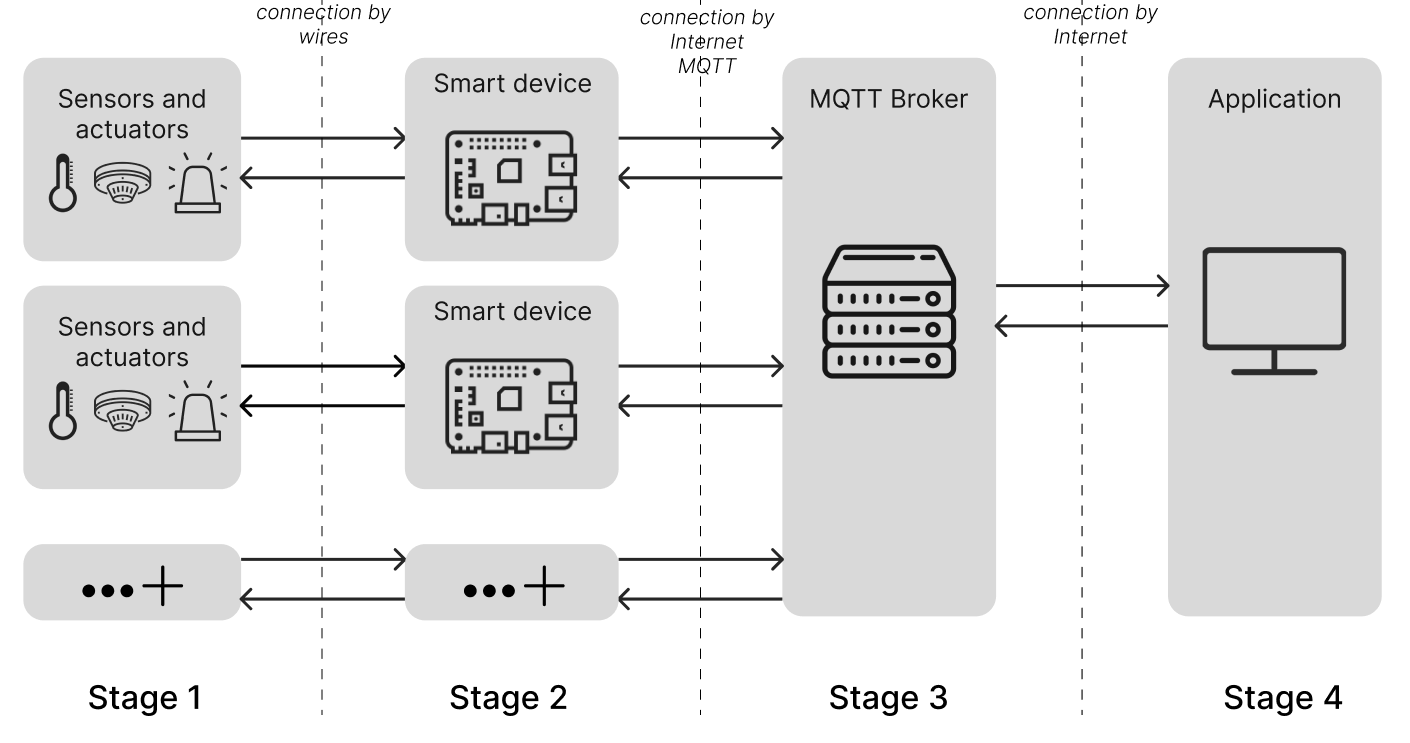
\includegraphics[width=.9\textwidth]{figures/proekt}
    \caption{Koncepcia architektonického modelu projektu \label{proekt}}
\end{figure}
Na obrázku \ref{proekt} si môžete podrobnejšie pozrieť môj koncept. Myslím si, že takéto pomerne štandardné a jednoduché architektonické riešenie bude pre študentov najvhodnejšie na učenie.

%%---------------------------------------------------------------

\subsection{Výber témy pre projekt}
Po vytvorení konceptu som začal premýšľať o konkrétnej téme projektu, ktorá by zodpovedala schéme na obrázku 2. Po dlhom premýšľaní a konzultácii s učiteľom som prišiel s nápadom vytvoriť systém na riadenie mikroklímy skleníkov. 

Podstatou tohto systému je zber údajov o teplote a vlhkosti v skleníkoch, analýza zozbieraných údajov a v prípade, že teplota alebo vlhkosť je mimo normy, potom sa mikroklíma skleníka riadi pomocou aktuátorov, ktoré uvedú ukazovatele do normálu.

Systém sa skladá z nasledujúcich komponentov:
\begin{itemize}
    \item Inteligentné zariadenie, ktoré je umiestnené v skleníku. Jeho úlohou je zber údajov o mikroklíme pomocou senzorov a ich analýza. Ak sú zozbierané údaje mimo normy, zariadenie aktivuje akčne členy, ktoré vyrovnávajú klímu. Všetky zozbierané údaje zo snímačov sa odosielajú na server.
    \item \gls{mqtt} broker, ktorý prijíma údaje, ich prenáša do webovej aplikácie.
    \item Webová aplikácia, ktorá umožňuje regulovať mikroklímu v každom skleníku a zobrazovať aktuálnu teplotu a vlhkosť.
\end{itemize}
Na prvý pohľad je táto myšlienka dobrá a dobre zapadá do koncepcie architektonického modelu (obr. \ref{proekt}), ale zdá sa to tak len na prvý pohľad. Problémy sa začínajú vo fáze rozšírenia implementácie projektu v školách. Teoreticky tento projekt obsahuje nielen senzory, ale aj akčné členy na zmenu teploty a vlhkosti. 

So senzormi by nemali byť žiadne problémy, potrebujeme len senzory svetla a vlhkosti (\gls{ldr} a \gls{dht}) a tie sú už dostupné v štandardných súpravách \textit{Arduino Kit}. Ale s akčnimy členamy je to úplne iná záležitosť. Pri analýze existujúcich riešení podobných nášmu projektu\cite{sklenik1} \cite{sklenik2} \cite{sklenik3}som si uvedomil, že na realizáciu tohto projektu by som potreboval nasledujúce pohony:
\begin{enumerate}
    \item Elektrický motorček (minimálne 12V) na zdvíhanie a spúšťanie okienka.
    \item Počítačový ventilátor na vetranie skleníka.
    \item Elektrické vodné čerpadlo na zvlhčovanie pôdy skleníka.
\end{enumerate}
Tieto komponenty už nie sú súčasťou súpravy \textit{Arduino Kit}, takže školy si budú musieť tieto nástroje zakúpiť dodatočne, čo pre nás nie je veľmi výhodné. Koniec koncov, jednou zo zásad, ktoré chcem pri tvorbe projektu dodržiavať, je minimalizovať dodatočné finančné náklady na kurz. 

Ďalším problémom pri vývoji tohto systému je náročnosť jeho implementácie v školách. Predstavme si, že 20 študentov absolvuje kurz a implementovalo systém podľa návodu. A teraz, aby ste tento systém otestovali, musíte sa veľmi snažiť, pretože školy zvyčajne nemajú niekoľko skleníkov. Samozrejme, môžete sa pokúsiť otestovať systém v rámci jednej alebo viacerých tried, ale podľa môjho názoru je to dosť náročná úloha. 

Vzhľadom na všetky uvedené nevýhody som si uvedomil, že myšlienka vyvinúť systém riadenia klímy v skleníku \gls{iot} nie je relevantná. Myslel som si však, že základ koncepcie je celkom zaujímavý, a tak som na základe predchádzajúcej myšlienky vytvoril novú, ktorá vyriešila všetky predchádzajúce problémy. 

Po niekoľkých ďalších konzultáciách a premýšľaní o možných riešeniach som prišiel s vhodnou myšlienkou bez zjavných nevýhod. Podstatou nového konceptu je vyvinúť systém zberu dát o počasí.

Systém pozostáva z niekoľkých meteorologických staníc navrhnutých študentmi, servera, ktorý zbiera údaje z týchto meteorologických staníc, a webovej aplikácie, z ktorej si môžete pozrieť všetky zozbierané údaje v grafoch, tabuľkách atď. Meteorologická stanica meria teplotu, vlhkosť a svetlo.

Ako vidíte, tento systém je zjednodušenou verziou predchádzajúceho systému. Ako som už napísal vyššie, od predchádzajúcej myšlienky som sa nevzdialil a jednoducho som odstránil komponenty, ktoré s ňou kolidovali, podľa logiky žiadne komponenty, žiadne problémy. Pri analýze predchádzajúceho riešenia som si uvedomil, že hlavným problémom boli pohony, pretože tie projekt úmerne komplikovali. Preto nové riešenie už nemá žiadne pohony, má len najjednoduchšie snímače, ktoré nie je potrebné dokupovať do škôl. 

Napriek tomu, že nové riešenie je trochu zjednodušené, nemyslím si, že by to mohlo nejako ovplyvniť kvalitu vedomostí poskytovaných žiakom. Práve naopak, zjednodušenie hardvéru projektu nám umožní venovať viac pozornosti programovaniu a spracovaniu zozbieraných údajov. Podľa môjho názoru práve toto bude pre mladých programátorov v oblasti internetu vecí užitočnejšie. 
Kvôli prehľadnosti na záver zhrňme tému projektu.

Téma projektu:  Systém na zber údajov o počasí.
Architektúra projektu podľa mojej koncepcie (obr. \ref{proekt}):
\begin{itemize}
    \item Prvá fáza: Senzory tepla, vlhkosti a svetla (\gls{dht}/22, \gls{ldr})
    \item Druhá fáza: Inteligentné zariadenie (ESP32/Raspberry pi)
    \item Tretia fáza: Server, ktorý slúži ako \gls{mqtt} broker
    \item Štvrtá fáza: Webová aplikácia, ktorá zobrazuje všetky zozbierané údaje.
\end{itemize}
Chcem poznamenať, že toto je len teoretický koncept, konečný výsledok sa môže počas vývoja dopĺňať a meniť.

%%---------------------------------------------------------------

\subsection{Výber softvéru a hardvéru na školenie}
Pri čítaní predchádzajúcej časti ste si možno všimli, že použitie takých dosiek ako \textit{ESP32} alebo \textit{Pasbery Py 3/Pico} v projekte môže byť nevhodné a lepším riešením by bolo nahradiť ich \textit{Arduino Uno}. Koniec koncov, \textit{Arduino Uno} je už v školách dostupné, takže nemusíte kupovať nič iné a nebudete musieť študentom vysvetľovať základy používania tohto zariadenia, pretože s ním už pracovali.

A ak vezmeme do úvahy len vyššie uvedené faktory, \textit{Arduino} vyzerá naozaj výhodnejšie v porovnaní s mikrokontrolérmi ako \textit{ESP32} alebo \textit{Raspberry Pi 3/Pico}. Aby som bol úprimný, na začiatku tejto práce som bol tiež fanúšikom používania \textit{Arduina}. V tejto časti však dokážem, prečo bude výber dosky \textit{ESP32} albo \textit{Pasbery Py 3/Pico} v tejto práci vhodnejší, ako rodina dosiek \textit{Arduino}.

Prvá vec, ktorú je potrebné si uvedomiť, je, že vo väčšine štandardných mikrokontrolérov (napr. \textit{ESP32}, \textit{Raspberry Pi 4}, \textit{Raspberry Pi Pico}) už má zabudovaný WiFi modul, zatiaľ čo bežné \textit{Arduina} ho nemajú a preto ich bude treba kúpiť samostatne. Na internete som našiel len niekoľko modelov \textit{Arduina} s integrovaným WiFi modulom, ako napríklad \textit{ARDUINO UNO WiFi REV2}\footnote{\textit{https://store.arduino.cc/products/arduino-uno-wifi-rev2}} a \textit{Arduino Nano RP2040}\footnote{\textit{https://store.arduino.cc/products/arduino-nano-rp2040-connect}}. Avšak v súčasnosti sú tieto zariadenia buď rovnako drahé ako napríklad \textit{ESP32}, alebo niekedy aj drahšie.

Ďalším faktom v prospech doskam tipu \textit{ESP32} je základný programovací jazyk. V prípade rodiny \textit{Arduino} ide zvyčajne o jazyk \textit{C++}, zatiaľ čo u mikroprocesorov je to \textit{Micropython} (takže ten istý \textit{Python}, len s menšou funkcionalitou). Podľa mňa je to dosť dôležitý parameter pre ľahkosť vývoja. Každý, kto už niekedy programoval v jazyku \textit{Micropython}, môže potvrdiť, že programovanie v porovnani s \textit{C++} je oveľa jednoduchšie. Väčšina stredoškolákov už dobre ovláda \textit{Python}, takže programovanie v \textit{Micropythone} by nemalo byť komplikované. Bohužiaľ, v súčasnosti nie sú všetky dosky rodiny \textit{Arduino} podporované \textit{Micropythonom}\footnote{\textit{https://docs.arduino.cc/learn/programming/arduino-and-python}}, existujú len niektoré samostatné platformy, ktoré to môžu. Tieto zariadenia môžete vidieť na obrázku \ref{arduino}. Ako vidíte, v tomto zozname nie je najrozšírenejší Arduino Uno.
\begin{figure}[!ht]
    \centering
    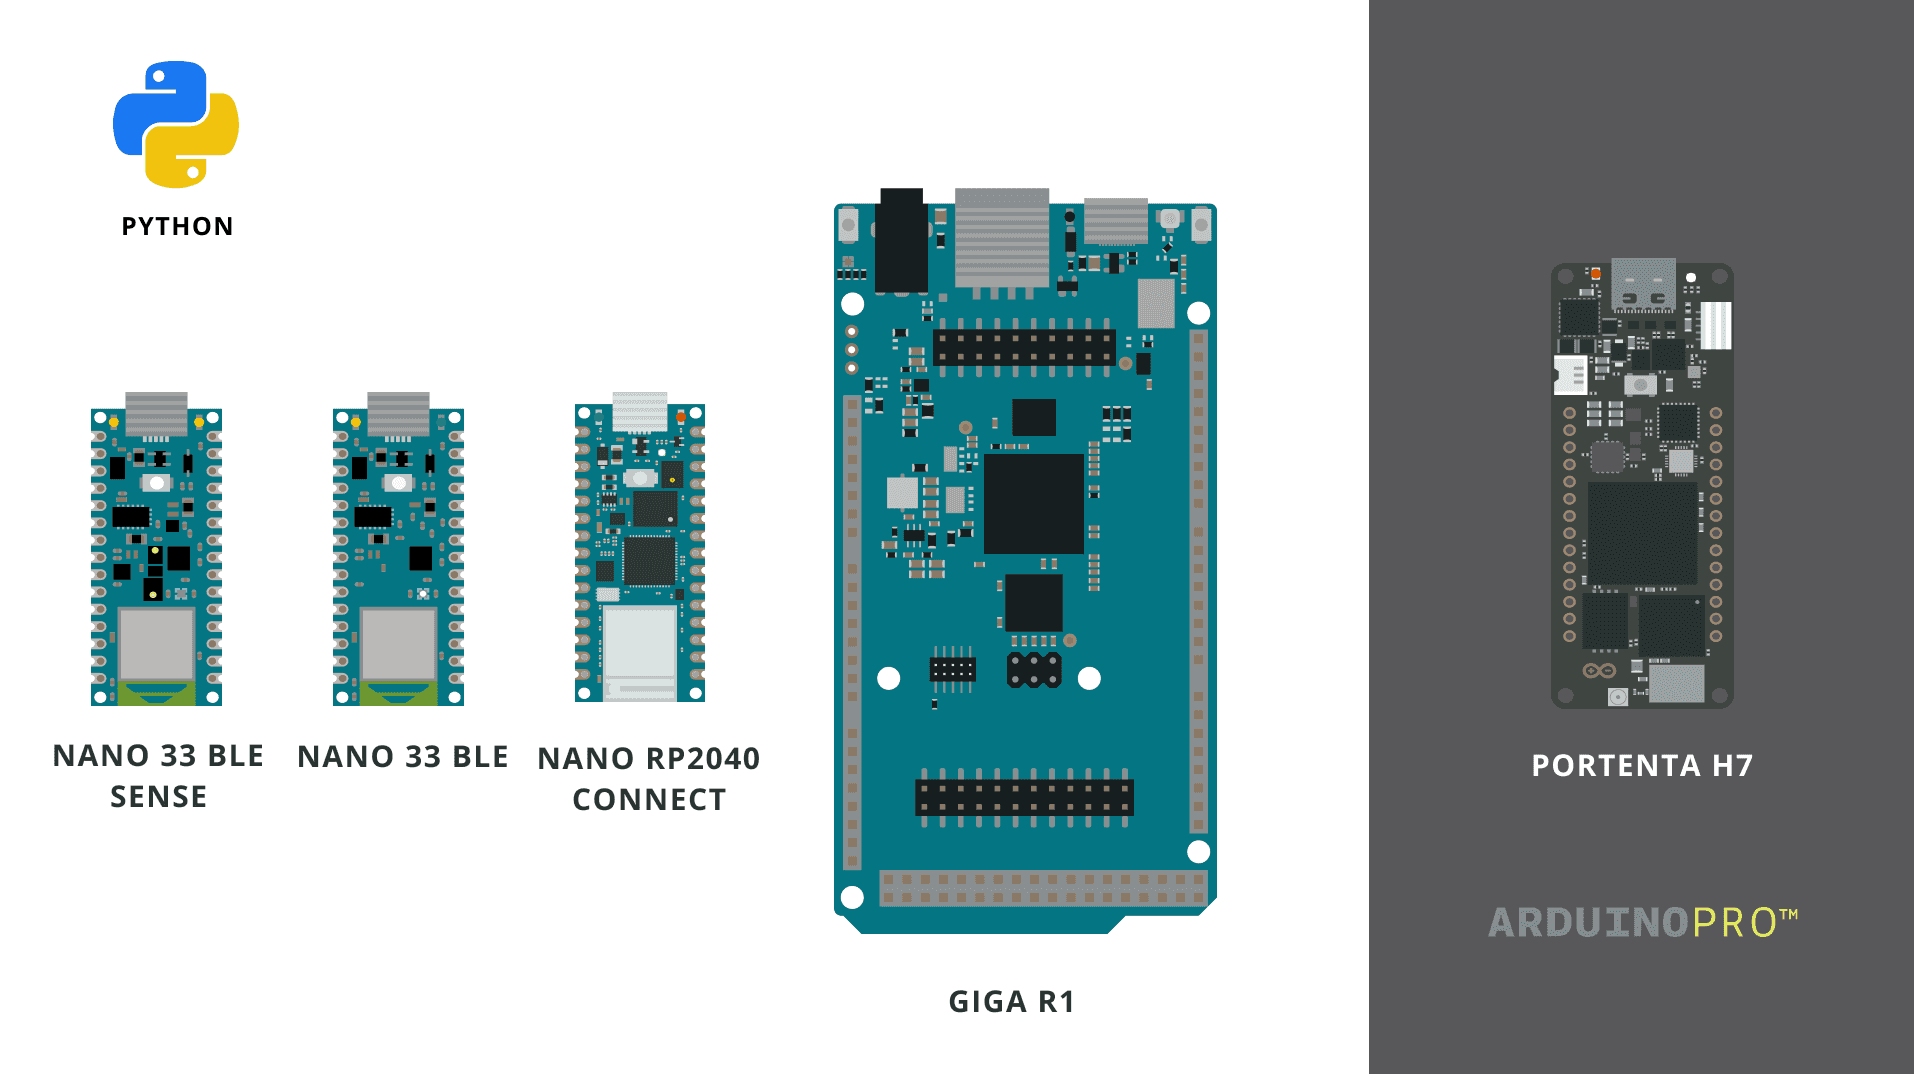
\includegraphics[width=.9\textwidth]{figures/arduino.png}
    \caption{Zoznam platforiem skupiny Arduino, ktoré podporujú Micropython \label{arduino}\cite{arduinoPyt}}
\end{figure}

Chcel by som ešte dodať, že dosky tipu \textit{ESP32} môžu vykonávať širší rozsah úloh než mikrokontroléry, preto výber mikroprocesora ako hlavného zariadenia pre programovanie umožní vyniesť zručnosti študentov na novú úroveň a v budúcnosti budú schopní vykonávať zložitejšie úlohy.


%%---------------------------------------------------------------

\subsection{Výber modelu mikrokontroléra}
Vzhľadom na špecifiká projektových podmienok som hodnotil model mikrokontroléra podľa nasledujúcich kritérií:
\begin{itemize}
    \item Jednoduchosť použitia
    \item Nízka cena
    \item Dostupnosť
\end{itemize}
Ďalším dôležitým parametrom, ktorý by mal byť jednoznačne zahrnutý v doske, je zabudovaný Wi-Fi modul. Zariadenia bez tohto parametru nebudú zvažované. Neberiem do úvahy samostatné čipy, ktoré nie sú pripojené k doske, pretože nie sú absolútne praktické pre prácu s žiakmi stredných škôl.

Ďalej podrobnejšie zanalyzujem jednotlivé kritériá a vyberiem najlepší motel dosky s mikroprocesorom. Začneme s dostupnosťou. Dostupným mikroprocesorom považujem ten, ktorý je ľahko dostupný na globálnom trhu. To znamená model, ktorý nie je deficitný alebo vzácny a je možné ho bez prekážok kúpiť na populárnych internetových obchodoch, ako sú \textit{alza.sk} alebo \textit{aliexpress.com}. Podľa tohto parametra môžem vyzdvihnúť nasledujúce dosky: \textit{ESP32}, \textit{Raspberry Pi 3/4}, \textit{Raspberry Pi Pico W}, \textit{ESP8266}. Na základe svojich skúseností môžem povedať, že najdostupnejšou a najpopulárnejšou voľbou je \textit{ESP32}.

Nasledujúcim kritériom je jednoduchosť použitia. Považujem za logické, ak dáme študentam zariadenie, ktoré bude najviac podobné tomu, čo už poznajú (v tomto prípade \textit{Arduino Uno}). Najvýhodnejšie na tomto poli vyzerá \textit{Raspberry Pi Pico W}, pretože z môjej skúsenosti môžem povedať, že toto zariadenie má najjednoduchšiu prvotnú konfiguráciu zo všetkých modelov, ktoré poznám. Okrem toho, komunikácia s týmto zariadením prebieha cez sériový port, rovnako ako u \textit{Arduino Uno}. Podobné charakteristiky v tejto oblasti má aj \textit{ESP32}, ale treba si uvedomiť, že pre tejto model existuje veľa rôznych konfigurácií, a môj projekt potrebuje štandardizované dosky

Nakoniec sme sa pozreli na otázku ceny. V súčasnosti najlacnejšími modelmi, ktoré som skúmal vyššie, sú \textit{ESP32} (10,81 €)\footnote{\textit{https://rpishop.cz/esp32-a-esp8266/3884-dfrobot-firebeetle-2-esp32-e-iot-mikrokontroler-s-podporou-wi-fi-bluetooth.html}}, \textit{ESP8266} (7,59 €)\footnote{\textit{https://rpishop.cz/esp32-a-esp8266/1944-nodemcu-esp8266-wifi-vyvojova-deska.html}}, \textit{Raspberry Pi Pico W} (7,59 €)\footnote{\textit{https://rpishop.cz/raspberry-pi-pico/5073-raspberry-pi-pico-w-5056561803173.html}}. Všetky ceny som bral z online obchodu \textit{"rpishop.cz"}\footnote{\textit{https://rpishop.cz/}}, pretože tam sú, podľa môjho subjektívneho názoru, dostatočne primerané ceny.

Po zhodnotení všetkých týchto parametrov som dospel k záveru, že Raspberry \textit{Pi Pico W} je najoptimálnejšou voľbou pre túto prácu.

%%---------------------------------------------------------------

\subsection{Dodatočné periférie pre Raspberry Pi Pico W}
Počas jednej z konzultácií mi bolo odporučane pre potreby prace použiť sa na pomocný prvok pre \textit{Raspberry Pi Pico W} s názvom \textit{Cytron Maker Pi Pico Base}\footnote{\textit{https://rpishop.cz/pico-karty/3854-cytron-maker-pi-pico-base-deska-pro-pi-pico-pro-zacatecniky-38515758.html}} (obr. \ref{piPlata}). Ide o pomocnú dosku, ktorej účelom je zjednodušiť pripojenie externých modulov. Skúšal som túto dosku pri vývoji meteorologickej stanice a môžem potvrdiť, že táto pomocná doska skutočne šetrí čas a nervy.

Hlavnou nevýhodou však je, že táto doska je dosť draha, konkrétne 11,02 € za kus. Okrem toho je potrebné dokúpiť špeciálne káble pre pripojenie modulov. Napriek zvýšeniu nákladov projektu, čo je v rozpore s mojím princípom ekonomického prístupu, implementujem túto dosku do kurzu, ale pridám aj možnosť nepoužívať ju na zlacnenie konečného výsledku.

\begin{figure}[!ht]
    \centering
    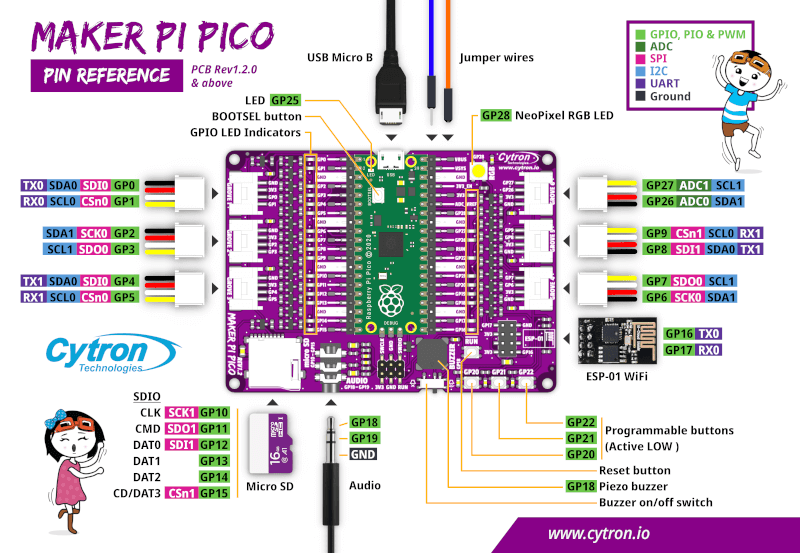
\includegraphics[width=.9\textwidth]{figures/piPlata.png}
    \caption{Vihlad \textit{Cytron Maker Pi Pico Base} \label{piPlata}\cite{cytron}}
\end{figure}

\subsection{Výber \gls{mqtt} brokera}
Zo svojich skúseností s vývojom riešení \gls{iot} môžem povedať, že technológie Hivemq\footnote{\textit{https://www.hivemq.com/}} a Mosquito\footnote{\textit{https://mosquitto.org/}} sú medzi vývojármi najobľúbenejšie. Preto pokladám za logické používať tieto \gls{mqtt} broukery. Ak tieto dve služby zoberieme do úvahy z hľadiska vývoja nášho produktu \gls{iot}, nie je medzi nimi veľký rozdiel. Existuje len malá výhoda Hivemq v podobe príťažlivejšieho webového rozhrania. 

Pri príprave tejto kapitoly som sa zoznámil s študentom Šimonom Pavlišinom, ktorého bakalársky projekt sa týkal vývoja \gls{iot} Gateweja a služby \gls{mqtt} brokera. 

Jeho projekt sa volá \textit{Otvorený \gls{iot} Lab pre stredné školy}\cite{bookSimon} a vyvíja v ňom \textit{Gateway}(ďalej GW) založenú na technológii Mosquito. 

Tento projekt má niekoľko zaujímavých vlastností:
\begin{itemize}
    \item Samotná aplikácia brokera je nainštalovaná na \textit{Raspberry Pi} tretej alebo štvrtej verzie a beží autonómne. Čiže pre lepšie pochopenie si tento projekt môžete predstaviť ako wifi router, ktorý funguje v rámci jedného laboratória alebo učebne, ale namiesto distribúcie wifi slúži ako \gls{mqtt} broker.
    \item Ďalšou vlastnosťou je, že na tomto GW možno vytvárať rôzne aplikácie, ktoré budú bežať paralelne. To sa dosiahne pomocou Doker\footnote{\textit{https://www.docker.com/}} kontajnerov. 
\end{itemize}
Po oboznámení sa s koncepciou projektu Šimona Pavlišina a otestovaní jeho raného prototypu som si uvedomil, že je to presne to, čo potrebujem pre svoju prácu. 

Pre väčšiu istotu uvediem nasledujúce argumenty:
\begin{enumerate}
    \item Možnosť paralelného behu mnohých aplikácií na jednom GW je veľmi silným argumentom pri školení mnohých ľudí.
    \item Už pri práci s raným prototypom tohto projektu som bol presvedčený o jeho použiteľnosti.
    \item Keďže tento GW podporuje Docker, môžem na programovanie aplikácie svojho projektu použiť nastroj NodeRed. Výhody tohto nastroja oproti iným možnostiam opíšem v nasledujúcej časti.
\end{enumerate}
\subsection{Prečo NodeRed?}
Na základe mojich skúseností môžem povedať, že programovanie pmomcou nastroja NodeRed je jedno z najjednoduchších vo svojej oblasti. 

Myslím si, že pri vývoji aplikácie, ktorá je na štvrtej úrovni, je potrebné, aby táto fáza bola čo najjednoduchšia a najľahšia. Podľa môjho názoru je to totiž jedna z najťažších fáz vývoja a myslím si, že ak túto časť príliš skomplikujete, bude materiálu na 5 prednášok príliš veľa. Preto si myslím, že NodeRed bude najjednoduchší a najnázornejší spôsob, ako to urobiť.
